\documentclass[12pt,a4paper]{article}
\usepackage[utf8]{inputenc}
\usepackage[russian]{babel}
\usepackage{amsmath}
\usepackage{amsfonts}
\usepackage{amssymb}
\usepackage{graphics}
\usepackage[pdftex]{graphicx}
\usepackage{lscape}
\usepackage{listings}
\usepackage{geometry} % Меняем поля страницы
\geometry{left=2cm}% левое поле
\geometry{right=1.5cm}% правое поле
\geometry{top=2cm}% верхнее поле
\geometry{bottom=15mm}% нижнее поле
\RequirePackage{float}
\renewcommand{\baselinestretch}{1.5}
\pagestyle{plain}
\begin{document}
\thispagestyle{empty}
\begin{center}
\large Санкт-Петербургский государственный политехнический университет\\
Институт информационных технологий и управления\\
Кафедра компьютерных систем и программных технологий\\
\vspace{60mm}
\Large Курсовая работа \\ По предмету "Проектирование архитектур программного обеспечения" \\на тему:\\
\LARGE\textbf{Создание информационной систеы}
\end{center}

\vspace{35mm}
\begin{flushright}
\large Выполнила: студентка группы 53501/3\\ Тарасова А. А.\\ Преподаватель: Зозуля А. В.
\end{flushright}
\vspace{30mm}

\begin{center}
Санкт-Петербург\\ 2015
\end{center} % это титульный лист
\newpage
\tableofcontents
\newpage
\section{Сбор функциональных требований}
Разрабатываемая информационная система является сервисом, позволяющим просматривать предложениях об экскурсиях по Санкт-Петербургу, бронировать экскусии, а так же следить за текущими предложениями экскурсоводов.

\textbf{Пользователями системы могут быть:}
\begin{itemize}
\item \textbf{Клиенты} - обычные пользователи, которые хотят воспользоваться разрабатываемой информационной системой для выбора и заказа самых разнообразных экскурсий.
\item \textbf{Экскурсоводы} - пользователь, который может предложить экскурсии.
\item \textbf{Администратор}  -  пользователь, который занимается проверкой всей поступившей информации, модерацией, добавлением и редактированием персональных данных.
\end{itemize}
\subsection{Функциональные требования для клиента}
\begin{itemize}
\item Просмотр полного списка экскурсий с их описанием
\item Бронирование экскурсии
\item Внесение предоплаты за экскурсию
\item Отмена брони экскурсии
\end{itemize}
\subsection{Функциональные требования для экскурсовода}
\begin{itemize}
\item Просмотр полного списка экскурсий с их описанием
\item Добавление экскурсий и их описания
\end{itemize}
\subsection{Функциональные требования для администратора}
\begin{itemize}
\item Просмотр полного списка экскурсий с их описанием
\item Модерация экскурсий, добавленных экскурсоводом
\item Размещение и удаление экскурсий 
\end{itemize}
\newpage
\section{Разработка вариантов использования (обобщенная диаграмма прецедентов)}
\subsection{Варианты использования. Пользователь Клиент}
\begin{enumerate}
\item Просмотр полного списка экскурсий с их описанием
\begin{enumerate}
\item При запуске программы пользователь проходит авторизацию как \textit{гость}
\item Пользователь использует функцию \textit{список экскурсий}
\item Система отображает список со всеми экскурсиями и их описанием
\end{enumerate}
\item Бронирование экскурсии
\begin{enumerate}
\item При запуске программы пользователь проходит авторизацию как \textit{гость}
\item Пользователь использует функцию \textit{список экскурсий}
\item Система отображает список со всеми экскурсиями и их описанием
\item Пользователь использует функцию \textit{забронировать экскурсию}
\item Система отображает сообщение, что экскурсия экскурсия будет забронирована после внесения предоплаты
\end{enumerate}
\item Внесение предоплаты за экскурсию
\begin{enumerate}
\item При запуске программы пользователь проходит авторизацию как \textit{гость}
\item Пользователь использует функцию \textit{список экскурсий}
\item Система отображает список со всеми экскурсиями и их описанием
\item Пользователь использует функцию \textit{забронировать экскурсию}
\item Система отображает сообщение, что экскурсия будет забронирована после внесения предоплаты
\item Пользователь использует функцию \textit{внести предоплату} и указывает данные для оплаты, имя пользователя и пароль.
\item Система выводит сообщение, что экскурсия забронирована..
\end{enumerate}
\item Отмена брони экскурсии
\begin{enumerate}
\item При запуске программы пользователь проходит авторизацию как \textit{пользователь}
\item Пользователь использует функцию \textit{Мои экскурсии}
\item Система отображает список со всеми забронированными экскурсиями пользоваьеля и их описанием
\item Пользователь использует функцию \textit{отменить бронь экскурсии}
\item Система отображает сообщение, что в случае отмены брони менее чем за 48 часов - предоплата не возвращается.
\item Пользователь использует функцию \textit{согласен с условиями}
\item Система выводит сообщение, что бронь на экскурсию отменена и предоплата будет возвращена. В случае если пользователь решил отменить бронь менее чем за 48 часов до начала мероприятия - предоплата не возвращается.
\end{enumerate}
\end{enumerate}
\subsection{Варианты использования. Пользователь Экскурсовод}
\begin{enumerate}
\item Просмотр полного списка экскурсий с описанием
\begin{enumerate}
\item При запуске программы пользователь проходит авторизацию как \textit{гость}
\item Пользователь использует функцию \textit{список экскурсий}
\item Система отображает список со всеми экскурсиями и их описанием
\end{enumerate}
\item Добавление экскурсий и их описания
\begin{enumerate}
\item При запуске программы пользователь проходит авторизацию как \textit{экскурсовод}
\item Пользователь использует функцию \textit{предложить экскурсию}
\item Система отображает форму для заполнения
\item Пользователь использует функцию \textit{добавить экскурсию}
\item Система выводит сообщение, что экскурсия будет доступна после модерации.
\end{enumerate}
\end{enumerate}
\subsection{Варианты использования. Пользователь Администратор}
\begin{enumerate}
\item Просмотр полного списка экскурсий с описанием
\begin{enumerate}
\item При запуске программы пользователь проходит авторизацию как \textit{гость}
\item Пользователь использует функцию \textit{список экскурсий}
\item Система отображает список со всеми экскурсиями и их описанием
\end{enumerate}
\item Модерация экскурсий, добавленных экскурсоводами
\begin{enumerate}
\item Пользователь проходит авторизацию как \textit{администратор}
\item Пользователь использует функцию \textit{список предложенных экскурсий}
\item Пользователь использует функцию \textit{разместить экскурсию}
\end{enumerate}
\end{enumerate}
\subsection{Диаграмма прецедентов}
\begin{figure}[h!]
\centering
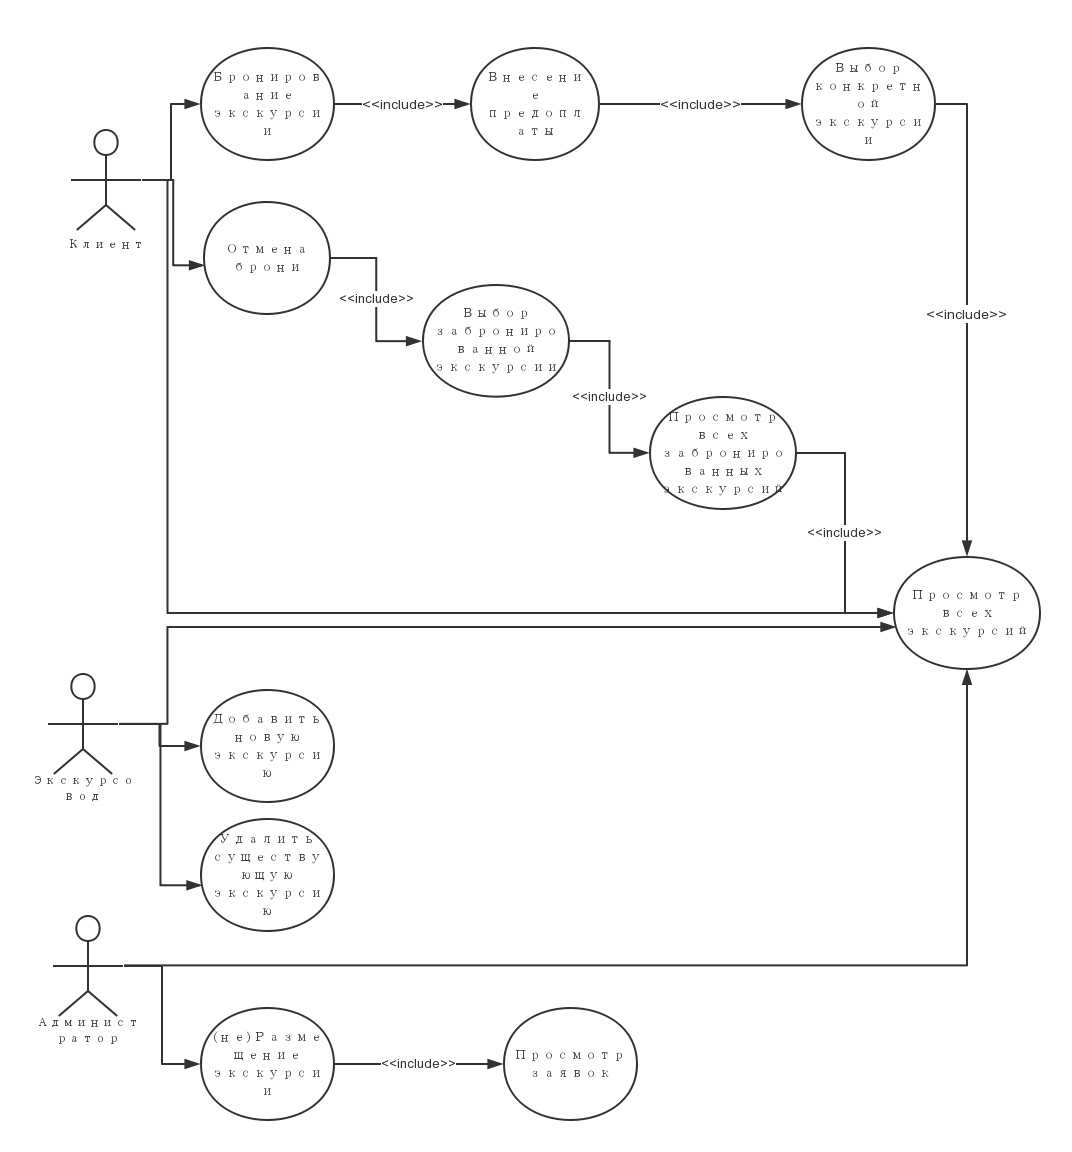
\includegraphics[scale=0.5]{res/usecase}
\caption{Диаграма прецедентов}
\end{figure}
\newpage
\section{Подробное описание всех вариантов использования (текстовое описание с альтернативами)}
\large \textbf{Заказ экскурсии}
\begin{enumerate}
\item Клиент просматривает список экскурсий и выбирает экскурсию для бронирования
\item Система выводит полную информацию о текущей экскурсии и ее цене
\item Клиент вводит информацию, необходимую для бронирования экскурсии: данные банковской карты, логин и пароль.
\item Система подтверждает оплату
\item Система отправляет клиенту и экскурсоводу контакты друг друга
\end{enumerate}

\textbf{Альтернатива}: постоянный клиент\\
Система выводит полную информацию о текущей экскурсии и ее цене, а также последние 4 цифры информации о банковской карточке
\newpage
\section{Разработка статической объектной модели предметной области (диаграммы классов)}
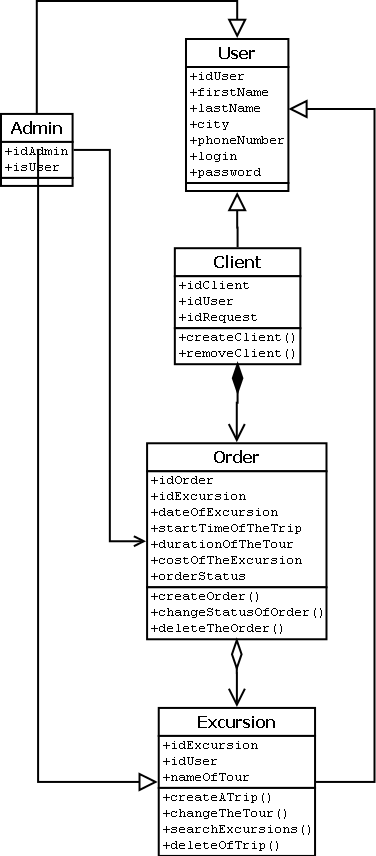
\includegraphics[scale=0.5]{res/class}
\caption{Диаграма классов}
\end{figure}
\section{Разработка динамической объектной модели предметной области (диаграммы последовательности)}
\section{Проектирование слоя бизнес-логики (выбор архитектурного шаблона уровня бизнес-логики)}
\section{Реализация слоя бизнес-логики (Java, NetBeans), unit-тестирование (JUnit)}
\section{Проектирование слоя источников данных (выбор архитектурного шаблона уровня доступа к данным: DB + внешний сервис)}
\section{Реализация слоя источников данных (JavaDB, NetBeans), unit-тестирование}

Таблица пользователей:
\begin{itemize}
\item idUser
\item userType
\item userName
\item numTelephone
\item e-mail
\end{itemize}

Таблица экскурсий:
\begin{itemize}
\item idExcursion
\item nameExcursion
\item descriptionExcursion
\item idGuide
\item status //null-не проводилась валидация, 1 - разрешено, 0 - не разрешено
\end{itemize}

Таблица клиент-экскурсия
\begin{itemize}
\item idRecord
\item idUser
\item idExcursion
\end{itemize}
\section{Проектирование сервисного слоя и слоя представления: GUI (Swing), внешний сервис}
\section{Реализация слоев представления, сервисного слоя, unit-тестирование сервисного слоя}
\section{Комплексное тестирование системы}
\end{document}